% Included by main.tex after \appendix; not a standalone document.
\section{Objective, derivatives, and interpretation}
\label{app:derivation}
This appendix derives the algebra used for candidate ordering. It introduces no new robustness theorem, approximation guarantee, or promise of an exact minimum-budget solver. Assumptions are finite fixed design vectors, outcomes in $[0,1]$, positive ridge $\lambda$, and the sum-loss objective in Eq.~\eqref{eq:objective}. Binary reversals additionally require distinct selected rows with original outcomes in $\{0,1\}$.

\subsection{Existence, uniqueness, and centering}
Each logistic contribution in Eq.~\eqref{eq:objective} is nonnegative for $y_i\in[0,1]$. Therefore $L(\theta;y)\geq\lambda\|\theta\|_2^2/2$, making the continuous objective coercive. A finite minimizer exists. With $p_i=\sigmoid(x_i^\top\theta)$,
\begin{equation}
\nabla L=\sum_i x_i(p_i-y_i)+\lambda\theta,\qquad
\nabla^2 L=\sum_i p_i(1-p_i)x_i x_i^\top+\lambda I\succeq\lambda I.
\label{eq:gradient}
\end{equation}
Strict convexity gives uniqueness, regardless of undirected graph connectivity. Connectivity is still reported because it characterizes the observed comparison design; ridge does not create empirical comparisons between disconnected components. Since $\mathbf{1}^\top x_i=0$, the first-order condition implies $\lambda\mathbf{1}^\top\hat\theta=0$. Thus the unique participant vector is centered without fixing an arbitrary participant to zero. This differs from an unregularized reference-coded BT maximum-likelihood fit.

\subsection{Flip-benefit sign}
For a prospective edit of row $i$, consider the continuous path $y_i(t)=y_i+t\delta y_i$, with $\delta y_i=1-2y_i$, holding all other rows fixed. Positive ridge ensures a nonsingular Hessian along this path. Differentiating the first-order condition at $t=0$ gives
\begin{equation}
H\frac{d\hat\theta(t)}{dt}\bigg|_{t=0}-x_i\delta y_i=0,
\qquad
\frac{d(c^\top\hat\theta(t))}{dt}\bigg|_{t=0}
=\delta y_i c^\top H^{-1}x_i.
\label{eq:implicit}
\end{equation}
Negating this derivative yields $B_i$ in Eq.~\eqref{eq:benefit}. A positive score predicts a decrease of the leader-minus-runner-up gap. For multiple edits the linear prediction is $\hat\Delta-\sum_{i\in\editset}B_i$; it neglects curvature changes. The path calculation is exact as a derivative, not as a finite-flip equality. Reported successes always use the refitted objective, not this prediction.

\subsection{Sufficient statistics and physical-row accounting}
Choose a canonical orientation for each unordered participant edge $e$, with vector $x_e$. Let $s_i=+1$ if row $i$ agrees with that orientation and $-1$ otherwise, and set $\tilde y_i=y_i$ or $1-y_i$, respectively. The aggregate objective is
\begin{equation}
\begin{aligned}
L(\theta)&=\sum_e\left[n_e\log(1+\exp(x_e^\top\theta))-w_e x_e^\top\theta\right]
+\frac{\lambda}{2}\|\theta\|_2^2,\\
n_e&=\sum_{i:e(i)=e}1,\qquad w_e=\sum_{i:e(i)=e}\tilde y_i.
\end{aligned}
\label{eq:aggregate}
\end{equation}
This equals the original-row objective, including ties. A selected decisive row changes $w_{e(i)}$ by $s_i(1-2y_i)$ and leaves $n_e$ unchanged. Aggregation reduces optimization work without changing the number of edited rows. Holding edge and canonical original-outcome edit counts fixed therefore fixes the modified sufficient statistics exactly. Ten concrete replacement checks per dataset in the implementation test this identity; they are not independent statistical evidence.

For the NBA home-adjusted sensitivity fit, replace $x_i$ by $(e_{u_i}-e_{v_i},h_i)$, with $h_i\in\{-1,0,1\}$ for away, neutral, and home. The parameter is $(\theta,\alpha)$ and the penalty is $\lambda(\|\theta\|_2^2+\alpha^2)/2$: the home coefficient is not exempt from ridge. Canonicalization reverses both the participant difference and $h_i$ when necessary. The margin vector is $(e_a-e_b,0)$. Aggregation then groups identical pair-and-home design rows, so the number of aggregate design rows need not equal the number of unordered participant edges. The participant block remains centered by the same argument as above.

\subsection{Search semantics and numerical verification}
All primary searches freeze the original pair and the initial positive-benefit ordering. Prefix fits start from the baseline solution, use damped Newton with backtracking, and allow at most 80 iterations. The target gradient infinity norm is $10^{-8}$, with a hard rejection threshold above $10^{-7}$. Search prefixes grow as powers of two up to the available list length or $\lfloor0.2N_{\rm dec}\rfloor$. Bisection retains an evaluated noncrossing lower endpoint and a crossing upper endpoint. It returns a neighboring transition; it does not assume or establish global monotonicity. A noncrossing $k-1$ does not exclude an earlier successful prefix or a different successful subset.

Saved original-row witnesses are reconstructed by changing their original labels and fitting a fresh BT object. \texttt{artifacts/witness\_verification.csv} records six passing checks, distinct decisive-edit counts matching Table~\ref{tab:main}, gradients below $2.7\times10^{-9}$, and agreement with stored refit gaps within $5.4\times10^{-11}$. These are numerical checks, not exact symbolic optimizations. Failures to find a witness remain unresolved, including if caused by the positive-benefit restriction, finite cap, or missed nonmonotone crossing.

\section{Data provenance, preprocessing, and target identities}
\label{app:data}
\begin{table}[htbp]
\centering
\caption{Data quality-control summary. For NBA, ``raw rows'' means the selected season's deduplicated game rows entering the audit, not every team-side record in the full historical source. Clusters are resampling units, not assertions of independence. Source: \texttt{artifacts/eda.csv}; generated input: \texttt{paper/tables/eda.tex}.}
\label{tab:eda}
{\small\begin{tabular}{lrrrr}
\toprule
Dataset & Raw rows & Used rows & Ties & Clusters \\
\midrule
Arena crowd & 57,477 & 57,477 & 17,761 & 57,477 \\
MT expert & 3,355 & 3,355 & 780 & 80 \\
MT GPT-4 & 2,400 & 2,400 & 600 & 80 \\
NBA 2013 & 1,314 & 1,314 & 0 & 1,314 \\
NBA 2014 & 1,319 & 1,319 & 0 & 1,319 \\
NBA 2015 & 1,311 & 1,311 & 0 & 1,311 \\
\bottomrule
\end{tabular}
}
\end{table}

\subsection{Parsing and retained observations}
Arena parsing reads only identifiers, participant names, and winner fields in chunks. Exactly one of the winner indicators must be active. The appearance threshold is evaluated on the released comparisons, and both participants must be eligible; all 64 participants pass in this snapshot. The full observed graph has 1,275 unordered edges. There are 39,716 decisive rows and 17,761 ties. IDs in all six prepared datasets are nonduplicated according to \texttt{eda.csv}.

For MT, observed winner labels map to $1$, $0$, or $1/2$. Unknown or missing mapped labels halt preparation. Human data contain 2,575 decisive rows and 780 ties. GPT data contain 1,800 decisive rows and 600 half-label rows, the latter comprising 380 inconsistent and 220 ordinary ties. Mapping inconsistent results to half labels is a modeling convention, not a claim that their underlying calls represent genuine preference ties. Both MT graphs include all 15 unordered edges among their six models. The question IDs supply 80 clusters per release. No reciprocal judging rows are manufactured.

The NBA source is checked for 63,157 unique game IDs over the full historical file. Keeping \texttt{\_iscopy==0} gives one row per game before selecting the three seasons. Each season has 30 teams and 435 observed unordered edges. We use the source's season-specific team codes, include playoffs, and do not pool years under a stationary team-strength assumption. All selected outcomes are decisive. The unadjusted primary BT model omits home and time effects; the separately labeled home sensitivity does not address all temporal nonstationarity.

The primary leading pairs are \texttt{gpt-4-1106-preview} versus \texttt{gpt-4-0125-preview} for Arena; \texttt{gpt-4} versus \texttt{claude-v1} for both MT releases; \texttt{MIA} versus \texttt{SAS} for NBA 2013; \texttt{SAS} versus \texttt{OKC} for NBA 2014; and \texttt{GSW} versus \texttt{HOU} for NBA 2015. Their direct exposures $D_{ab}$ are respectively 134, 200, 160, 9, 10, and 9 (\texttt{artifacts/baseline.csv}). These direct counts are distinct from union exposures in Table~\ref{tab:main}. The retained target names, rather than just their ranking positions, define the fixed-target ablations.

\subsection{Pinned sources and attribution}
\label{app:provenance}
The machine-readable manifest \texttt{data/manifest.json} supplies exact retrieval URLs, byte counts, licenses, and hashes. The access and literature statements in this manuscript describe existing local records; no new retrieval or search was performed to write it. The following are asset locators, not additional research-paper references.

\paragraph{Arena.}
Creator/host: \texttt{lmarena-ai}, dataset \texttt{arena-human-preference-55k}; license recorded as Apache-2.0. Commit:
\begin{quote}\small\path{18c298340948c0e7f7727399fd459cca6ce0ca6f}\end{quote}
Raw URL:
\begin{quote}\small\url{https://huggingface.co/datasets/lmarena-ai/arena-human-preference-55k/resolve/18c298340948c0e7f7727399fd459cca6ce0ca6f/train.csv}\end{quote}
SHA-256:
\begin{quote}\small\path{0692154aaf20fc6649090c3f49b6b5dd1e693a765ecb5f0856ae0da5946f5be2}\end{quote}
The associated evaluation platform is described by \citet{chiang2024chatbot}; the public snapshot is not assumed to equal their analysis snapshot or current production pipeline.

\paragraph{MT-Bench.}
Creator/host: \texttt{lmsys}, dataset \texttt{mt\_bench\_human\_judgments}; license recorded as CC-BY-4.0. The associated source is \citet{zheng2023judging}. Commit:
\begin{quote}\small\path{f7d2896d2cc5d80f8b55c2bbc722613555233c25}\end{quote}
Human URL and SHA-256:
\begin{quote}\small
\url{https://huggingface.co/datasets/lmsys/mt_bench_human_judgments/resolve/f7d2896d2cc5d80f8b55c2bbc722613555233c25/data/human-00000-of-00001-25f4910818759289.parquet}\\
\path{4877bc46a40929f4082c3c79593700fb897b1d6c7f4c473032694a01322f5769}
\end{quote}
GPT pair-result URL and SHA-256:
\begin{quote}\small
\url{https://huggingface.co/datasets/lmsys/mt_bench_human_judgments/resolve/f7d2896d2cc5d80f8b55c2bbc722613555233c25/data/gpt4_pair-00000-of-00001-c0b431264a82ddc0.parquet}\\
\path{57068327ffb5f8fddb15fedbbfe40b26fe862da2326331e5cf64a42320a00e71}
\end{quote}

\paragraph{NBA.}
Creator/host: FiveThirtyEight, repository \texttt{fivethirtyeight/data}, file \texttt{nba-elo/nbaallelo.csv}; license recorded as CC-BY-4.0. Commit:
\begin{quote}\small\path{4c1ff5e3aef1816ae04af63218015066e186c147}\end{quote}
Raw URL and SHA-256:
\begin{quote}\small
\url{https://raw.githubusercontent.com/fivethirtyeight/data/4c1ff5e3aef1816ae04af63218015066e186c147/nba-elo/nbaallelo.csv}\\
\path{d46ed3540ee8d9eca31b3e94cc8c777e0be5156173d814ebf65b8195e8d616bc}
\end{quote}
No NBA paper outside the allowed bibliography was consulted or added. Dataset attribution is provided directly rather than inventing a paper citation.

\section{Matching protocol and departures from the initial plan}
\label{app:matching}
The initial plan proposed separate reciprocal GPT judgments, possible soft-label averaging on matched cells, and a tentative Arena sample-size control. The observed files instead required exported GPT result units, one human row per ordered cell, and a corrected Arena target sample size. These are documented deviations, not silently equivalent implementations.

An ordered MT cell is the tuple (question ID, model A, model B, turn). \texttt{artifacts/matching\_protocol.json} records 2,396 human cells, 2,400 GPT cells, and 1,232 shared cells. GPT has one row on each retained cell. For seeds 100 through 119, human rows are grouped by cell and one row is sampled, then aligned to the same sorted GPT support. This varies the human judgment choice while holding the comparison support fixed. The GPT dataset is evaluated once. The local audit reports no answer-pair representation mismatch on the matched rows; this is not an independent upstream provenance audit or a correctness assessment of labels. Cell intersection excludes unmatched presentation orientations and may select an unrepresentative subset.

The Arena pool is induced by the full-fit top-six names: \texttt{gpt-4-1106-preview}, \texttt{gpt-4-0125-preview}, \texttt{gpt-4-0314}, \texttt{gpt-4-0613}, \texttt{qwen1.5-72b-chat}, and \texttt{mistral-medium}. From 3,222 eligible rows, each seed 100 through 119 samples 2,400 without replacement. Assertions and saved SHA-256 row-set identities establish 20 distinct subsets in the current artifacts. Subsets overlap and their cohort was selected using full-data outcomes. Targets are selected from each subset's fitted ranking, unlike fixed-target estimator ablations. These results therefore mix subset, target, margin, and cohort changes.

The earlier requested size of 3,355 exceeded the eligible pool. An initial implementation silently selected all 3,222 rows for each seed; those outputs are obsolete and excluded from every table and interpretation here. The historical \texttt{code\_audit.md} and \texttt{reflection.json} retain that earlier failure diagnosis; current acceptance evidence is \texttt{matching\_protocol.json}, \texttt{matched.csv}, and the corrected generated summaries. No independent-replicate uncertainty is assigned to either matching exercise.

\section{Resampling, Monte Carlo uncertainty, and secondary endpoints}
\label{app:uncertainty}
\subsection{Random controls and interval definition}
The control seed is $20261102+j$ and the bootstrap seed is $7300+j$, where $j=0,\ldots,5$ indexes Arena, MT human, MT GPT-4, NBA 2013, NBA 2014, and NBA 2015 in that order. Within each control trial, selected rows are distinct. Repeated draws can overlap. The controls sequentially consume a seeded random generator as implemented in \texttt{src/run.py}; the script, not an assumption of independent datasets, defines their reproducibility.

For $X$ successes in $n$ trials, with $\hat p=X/n$ and $z=1.959963984540054$, the pointwise two-sided 95\% Wilson interval has center and radius
\begin{equation}
 m=\frac{\hat p+z^2/(2n)}{1+z^2/n},\qquad
 r=\frac{z}{1+z^2/n}\sqrt{\frac{\hat p(1-\hat p)}{n}+\frac{z^2}{4n^2}},
 \qquad [m-r,m+r]\cap[0,1].
\label{eq:wilson}
\end{equation}
The interval describes Monte Carlo success probability under the specified random-subset mechanism conditional on the fitted dataset, target, and chosen budget. It is not uncertainty over future leaderboards. For $X=0,n=100$, its upper endpoint rounds to \ZeroUpper\%. No familywise or false-discovery correction was applied because no multiplicity-controlled inferential claim is made. These intervals must not be read as simultaneous coverage across the many panels and budgets. All full-precision control endpoints are in \texttt{artifacts/control\_summary.csv}.

\subsection{Empirical resampling is not fixed-schedule uncertainty}
\begin{table}[htbp]
\centering
\caption{Selected-target descriptive resampling summaries. Gap bands are empirical 2.5th and 97.5th percentiles over 200 draws, not selection-adjusted population intervals. Positive margin means the original leader exceeds the original runner-up by more than $10^{-7}$. ``Slot witnesses'' counts successful auxiliary searches among the first 30 draws; these are attempted only for positive original-pair margins and edit resampled slots, possibly duplicated original IDs. Source: \texttt{artifacts/uncertainty.csv}; generated input: \texttt{paper/tables/bootstrap.tex}.}
\label{tab:bootstrap}
{\small\begin{tabular}{lrrr}
\toprule
Dataset & Gap percentile band & Positive margin & Slot witnesses \\
\midrule
Arena crowd & [-0.103, 0.107] & 110/200 & 16/30 \\
MT expert & [0.137, 0.655] & 199/200 & 29/30 \\
MT GPT-4 & [0.555, 1.087] & 200/200 & 30/30 \\
NBA 2013 & [-0.479, 0.894] & 155/200 & 24/30 \\
NBA 2014 & [-0.387, 0.780] & 163/200 & 28/30 \\
NBA 2015 & [0.090, 1.269] & 199/200 & 29/30 \\
\bottomrule
\end{tabular}
}
\end{table}

For Arena and NBA, empirical resampling draws row counts from a multinomial distribution with as many draws as original rows. MT resamples question clusters, retaining all rows belonging to each selected question; total row count can then vary. Targets remain the original full-data pair, not the newly selected leading pair. Edges and their multiplicities change. The primary label-flip intervention remains fixed-schedule, but this resampling procedure does not.

The first 30 draws additionally recompute witnesses only when the original-pair margin is positive. A pseudodataset expands repeated rows into separate slots; two slots originating from one physical observation can be edited separately. Its budget is consequently not a budget over unique original IDs. Current outputs distinguish \texttt{already\_reversed}, \texttt{numerical\_tie}, \texttt{found\_on\_resampled\_slots}, \texttt{search\_failed}, and draws outside the first 30. The final column of Table~\ref{tab:bootstrap} is not 30 unconditional minimum-budget estimates, and missing searches are not numerical robustness lower bounds. Auxiliary slot-budget quantiles in the CSV summaries are supplementary exploratory statistics only; we do not use them as headline uncertainty or confidence intervals for physical-row attacks.

Dependence remains incompletely modeled. Arena resampling uses votes rather than users; NBA uses games without team/time block structure; MT question clusters do not capture every crossed judge dependence. More elaborate resampling would require additional assumptions and is not a correction that can be applied to the present bands by relabeling them.

\subsection{Supplementary dose responses}
\begin{figure}[htbp]
\centering
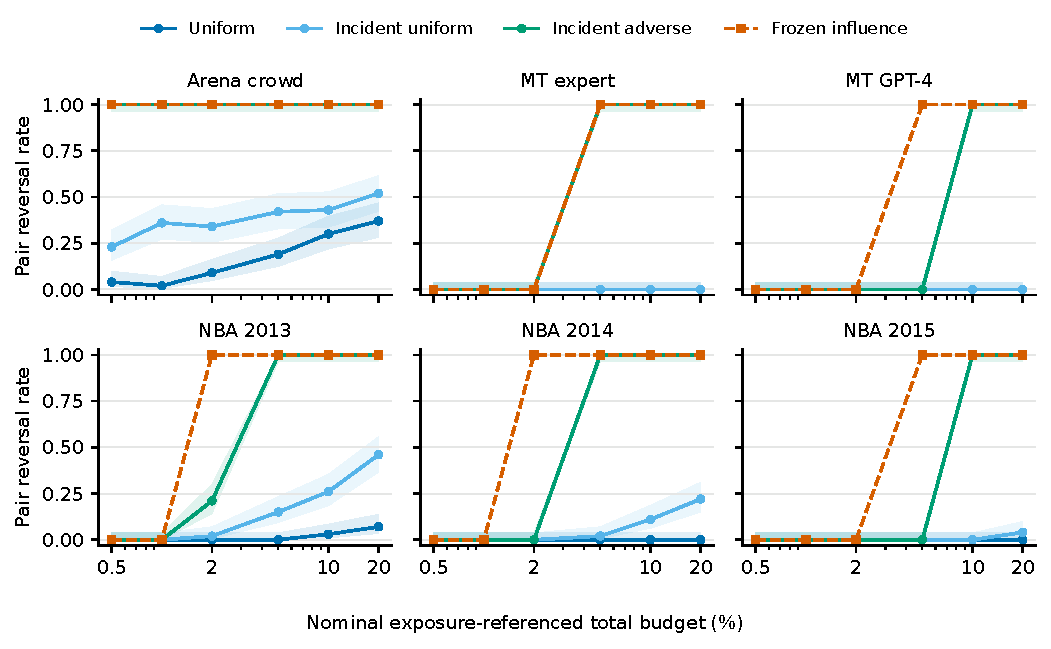
\includegraphics[width=\linewidth]{figures/dose_response.pdf}
\caption{Supplementary strict pair-reversal dose responses. Nominal fractions are $f\in\{0.005,0.01,0.02,0.05,0.1,0.2\}$ and actual integer budgets are $k=\max(1,\lceil fE_{ab}\rceil)$. The figure places points on the nominal grid, so plotted positions are not exact realized percentages after rounding. Random orderings are nested within a repeat, with 100 repeats; shaded bands are pointwise 95\% Wilson Monte Carlo intervals. Frozen influence has one deterministic ordering, not 100 replicates. Budgets exceeding an eligible ordering's length are omitted. Global controls can spend edits off-target, so the horizontal scale is exposure-referenced total cost, not always an incident-corruption fraction. Source: \texttt{artifacts/random\_curves.csv}; generated figure: \texttt{paper/figures/dose\_response.pdf}.}
\label{fig:dose}
\end{figure}

The dose-response grid is distinct from the primary powers-of-two witness search and its 20\%-of-decisive-rows cap. Secondary strict leader replacement is defined by $\max_j\theta_j>\theta_a+10^{-7}$. Secondary pair disagreement is the fraction of all unordered participant pairs whose fitted difference changes strict sign; pairs tied in either fit contribute zero. It is not a tie-corrected Kendall statistic. These metrics are logged in \texttt{random\_curves.csv}; no unsupported ranking-generalization claim is attached to them. The initial argmax-only winner-change metric could count ties; the corrected strict metric and its regression test supersede it.

\subsection{All adjacent baseline pairs}
\begin{figure}[htbp]
\centering
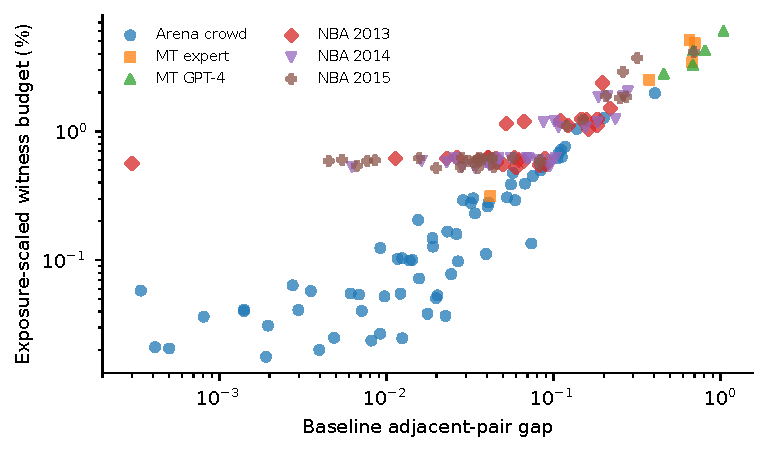
\includegraphics[width=0.85\linewidth]{figures/adjacent_pairs.pdf}
\caption{Secondary adjacent-pair audit: baseline gap versus exposure-scaled witness budget, both on logarithmic axes. The procedure audits \AdjacentCount{} adjacent pairs across the six baseline rankings. Points are selected-data descriptors; neither an association p-value nor a causal relationship is claimed. The same search incompleteness and denominator qualifications apply as for the primary audit. Source: \texttt{artifacts/adjacent.csv}; summaries: \texttt{artifacts/adjacent\_summary.csv}; generated figure: \texttt{paper/figures/adjacent\_pairs.pdf}.}
\label{fig:adjacent}
\end{figure}

The numbers of adjacent pairs follow the cohort sizes: 63 for Arena, five per MT release, and 29 per NBA season. Targets are selected from each baseline ordering; pair results share observations and are not independent tests. The CSV summaries include within-panel Spearman correlations as descriptive associations only. There is no selection-adjusted or multiplicity-corrected inferential claim for the most fragile pair, and the scatter is not evidence that gap alone determines edit budgets.

\section{Fixed-target estimator ablations}
\label{app:ablations}
\begin{table}[htbp]
\centering
\caption{Full fixed-target sensitivity results. Each row retains the corresponding primary target identities. The gap is before outcome edits under the changed estimator/data convention. $k=0$ with ``Already reversed'' means the specification change alone reverses the original pair, not a successful zero-edit attack on the primary specification. Other $k$ values are sufficient witnesses, not minima. Tie removal changes $N$ and $E_{ab}$; ridge alone does not. Source: \texttt{artifacts/fixed\_target\_ablations.csv}; generated input: \texttt{paper/tables/fixed\_ablations.tex}.}
\label{tab:ablations}
{\small\setlength{\tabcolsep}{4pt}\begin{tabular}{llrrl}
\toprule
Dataset & Change & Original-pair gap & $k$ & Status \\
\midrule
Arena crowd & $\lambda=0.1$ & 0.004 & 1 & Witness \\
Arena crowd & $\lambda=10$ & 0.044 & 11 & Witness \\
Arena crowd & Remove ties & -0.023 & 0 & Already reversed \\
MT expert & $\lambda=0.1$ & 0.378 & 46 & Witness \\
MT expert & $\lambda=10$ & 0.357 & 46 & Witness \\
MT expert & Remove ties & 0.527 & 42 & Witness \\
MT GPT-4 & $\lambda=0.1$ & 0.820 & 61 & Witness \\
MT GPT-4 & $\lambda=10$ & 0.724 & 61 & Witness \\
MT GPT-4 & Remove ties & 1.065 & 40 & Witness \\
MT GPT-4 & Remove inconsistent & 0.971 & 47 & Witness \\
NBA 2013 & $\lambda=0.1$ & 0.228 & 3 & Witness \\
NBA 2013 & $\lambda=10$ & 0.168 & 3 & Witness \\
NBA 2013 & Home covariate & 0.207 & 3 & Witness \\
NBA 2014 & $\lambda=0.1$ & 0.295 & 4 & Witness \\
NBA 2014 & $\lambda=10$ & 0.192 & 4 & Witness \\
NBA 2014 & Home covariate & 0.283 & 4 & Witness \\
NBA 2015 & $\lambda=0.1$ & 0.744 & 8 & Witness \\
NBA 2015 & $\lambda=10$ & 0.451 & 8 & Witness \\
NBA 2015 & Home covariate & 0.715 & 8 & Witness \\
\bottomrule
\end{tabular}
}
\end{table}

The primary $\lambda=1$ rows are in Table~\ref{tab:main}; Table~\ref{tab:ablations} supplies the changes around them. Ridge values 0.1 and 10 bracket the specified primary value without selecting a value for a preferred fragility result. On a sum loss, this is not a constant per-observation penalty across datasets or changing sample sizes. Removing all ties and excluding only GPT inconsistent rows test different conventions and have different denominators.

The earlier \texttt{artifacts/ablations.csv} reselects a leading pair after each change. That file is not used as evidence of same-target sensitivity. For example, reselecting the NBA 2015 runner-up can change both target identity and exposure; freezing identities avoids this conflation. A future result that is already reversed, numerically tied, or unresolved must keep that status rather than being replaced by a favorable newly selected pair. The present full fixed-target table includes the already-reversed Arena case explicitly.

\section{Adaptive flips and same-estimator deletion}
\label{app:comparators}
\begin{table}[htbp]
\centering
\caption{Supplementary method comparison on original targets. Adaptive flips refit and relinearize after every new edit; frozen flips use the initial ordering. Deletion removes rows under the same sum-loss ridge estimator. ``Linear prediction'' is the frozen first-order cumulative-budget prediction, not a verified finite edit result. Counts across interventions are not exchangeable and do not reproduce published deletion experiments. Sources: \texttt{artifacts/method\_comparison.csv} and \texttt{artifacts/baseline.csv}; generated input: \texttt{paper/tables/methods.tex}.}
\label{tab:methods}
{\small\begin{tabular}{lrrrr}
\toprule
Dataset & Frozen flips & Adaptive flips & Deletion & Linear prediction \\
\midrule
Arena crowd & 2 & 2 & 3 & 2 \\
MT expert & 46 & 46 & 92 & 45 \\
MT GPT-4 & 61 & 61 & 144 & 56 \\
NBA 2013 & 3 & 3 & 5 & 3 \\
NBA 2014 & 4 & 4 & 7 & 4 \\
NBA 2015 & 8 & 8 & 16 & 8 \\
\bottomrule
\end{tabular}
}
\end{table}

Adaptive selection recomputes flip benefits at each current optimum, chooses an available positive-benefit decisive row, never reuses a row, and refits the cumulative selected set against the original dataset. It uses the same target and decisive-row cap. The unchanged budgets in Table~\ref{tab:methods} provide no empirical improvement for this comparator on the six primary instances; neither procedure is an optimal solver.

For deletion, let $p_i$ be the original fitted probability. Infinitesimally removing row $i$ changes the margin by approximately $(p_i-y_i)c^\top H^{-1}x_i$, so the static harmful-deletion score is
\begin{equation}
 B_i^{\rm del}=-(p_i-y_i)x_i^\top H^{-1}c.
\label{eq:deletion}
\end{equation}
The implementation orders positive scores and searches deletion prefixes with full numerical refits, up to 20\% of original rows. Tie rows can have deletion influence even though they are ineligible for binary flips. Removal changes the comparison schedule and the likelihood information; a flip instead reverses an outcome while retaining its contribution to exposure. The penalty remains fixed in both procedures. Their count difference is an intervention comparison, not an efficiency ratio between algorithms and not a reproduction of \citet{huang2025dropping} or \citet{broderick2020automatic}. Their published snapshots, filtering choices, and estimators are not assumed to match ours.

\section{Reproduction instructions and artifact map}
\label{app:reproduction}
\subsection{Environment, commands, and measured resources}
The corrected main run records Python 3.11.15 on
\begin{quote}\small\path{Linux-7.0.0-38-generic-x86_64-with-glibc2.41}.\end{quote}
Dependencies used by the scripts include NumPy, pandas, SciPy, matplotlib, pyarrow, requests, and pytest. Numerical runs are CPU-only with \texttt{OPENBLAS\_NUM\_THREADS=1}, \texttt{OMP\_NUM\_THREADS=1}, and \texttt{MKL\_NUM\_THREADS=1}. The project's resource constraint was at most 8\,GB memory, at most 3\,GB data, and CPU-only operation; this is a constraint, not a measured peak-use claim. Visible CPU metadata and separately measured replay memory are reported below; visible host topology does not imply exclusive allocation.

The following commands reproduce the local-data path from the project root, here mounted at \texttt{/work}. They are documentation, not commands executed during manuscript drafting. Raw files must already exist at the four locations in \texttt{data/manifest.json} and match the listed hashes; these commands require no network access and do not infer new snapshots.
\begin{verbatim}
PYTHONPATH=/work/src python /work/src/prepare.py
OPENBLAS_NUM_THREADS=1 OMP_NUM_THREADS=1 MKL_NUM_THREADS=1 \
  PYTHONPATH=/work/src python -m pytest -q /work/tests
OPENBLAS_NUM_THREADS=1 OMP_NUM_THREADS=1 MKL_NUM_THREADS=1 \
  PYTHONPATH=/work/src python /work/src/run.py \
  --repeats 100 --bootstrap 200
OPENBLAS_NUM_THREADS=1 OMP_NUM_THREADS=1 MKL_NUM_THREADS=1 \
  PYTHONPATH=/work/src python /work/src/supplement.py
PYTHONPATH=/work/src python /work/src/report.py
\end{verbatim}
The last command regenerates tables, figures, \texttt{paper/numbers.tex}, and summary CSV/JSON files. It must follow the supplementary run because the report reads fixed-target ablations and comparator artifacts. The seven-test result in \texttt{artifacts/tests.log} is existing evidence, not a fresh test claimed by this writing pass. Script paths resolve their root from their own location rather than requiring a changed working directory.

\begin{table}[htbp]
\centering
\caption{Recorded per-dataset runtime instrumentation from the corrected main run. Fits count calls registered on each primary dataset's BT object; auxiliary bootstrap-pseudodataset, matching, and supplementary objects are not a complete project fit count. Seconds are measured per-dataset blocks, not hardware-normalized estimates. Gradient maxima are rounded. Source: \texttt{artifacts/runtime.csv}; generated input: \texttt{paper/tables/runtime.tex}.}
\label{tab:runtime}
{\small\begin{tabular}{lrrr}
\toprule
Dataset & Fits & Seconds & Max $\|g\|_\infty$ \\
\midrule
Arena crowd & 2691 & 17.77 & 1e-08 \\
MT expert & 2479 & 2.21 & 1e-08 \\
MT GPT-4 & 2481 & 2.41 & 9.8e-09 \\
NBA 2013 & 2455 & 3.96 & 1e-08 \\
NBA 2014 & 2458 & 4.02 & 9.9e-09 \\
NBA 2015 & 2468 & 4.21 & 9.5e-09 \\
\bottomrule
\end{tabular}
}
\end{table}

The corrected main script, including its ablation and matching stages, records \MainSeconds{} seconds elapsed. Table~\ref{tab:runtime} sums to \MainFitCount{} instrumented primary-object fit calls; its reported maximum gradient, rounded by the generator, is \texttt{\MaxGradient}. The separate supplement records approximately 3.46 seconds in \texttt{artifacts/supplement\_metadata.json}. Neither number includes all preparation, downloads, dependency installation, source reading, earlier failed or corrected runs, report rendering, or manuscript compilation. Total project compute was not fully metered; preliminary and failed runs are documented in \texttt{experiment\_log.md}. Dense Hessian storage scales quadratically and factorization cubically in participant count; the small cohorts here do not establish large-cohort scalability.

The visible CPU is an Intel Xeon Gold 6230 at 2.10\,GHz (\texttt{artifacts/hardware.txt}); the sequential numerical process uses one BLAS thread, not all visible host cores. A separately rooted replay in a newly created virtual environment installed \texttt{requirements.txt}: NumPy 2.4.6, SciPy 1.17.1, pandas 3.0.6, matplotlib 3.11.2, pyarrow 26.0.0, requests 2.34.2, pytest 9.2.0, pypdf 6.21.4, and threadpoolctl 3.7.0. Full transitive versions are in \texttt{artifacts/environment\_freeze.txt}. The replay's main run took 41.26 seconds and its child-process peak resident memory was 301.87\,MiB (Linux \texttt{resource.RUSAGE\_CHILDREN}; \texttt{artifacts/resource\_replay.json}). These measurements concern that replay only, not the complete project. All 13 deterministic result CSVs agree with the accepted run within $10^{-8}$ relative and $10^{-9}$ absolute tolerance; timing metadata is intentionally excluded. Seven tests also pass in the isolated environment. The replay shares checksummed raw files but runs relocated source code and a separately installed Python environment. It is not an independent data collection. A complete, copy-safe validation command from the project root is
\begin{verbatim}
PYTHONPATH=src python src/validate.py --replay reproduction_check
\end{verbatim}
The directory argument is the actual replay root; creation, installation, measurement and output comparison are documented in the accompanying README.

\subsection{Mapping reported outputs to source artifacts}
All tabular inputs and numerical figures are generated by \texttt{src/report.py}, not manually reconstructed in this manuscript. PDF and PNG figures with the same basename are available in \texttt{paper/figures/}.
\begin{itemize}
\item Table~\ref{tab:main}: \texttt{artifacts/baseline.csv} to \texttt{paper/tables/main.tex}; row-level evidence in \texttt{witness\_rows.csv} and \texttt{witness\_verification.csv}.
\item Figure~\ref{fig:budget}: \texttt{baseline.csv} and \texttt{uncertainty.csv} to \texttt{paper/figures/budget\_and\_margin.pdf}.
\item Table~\ref{tab:controls}: \texttt{controls.csv} to \texttt{control\_summary.csv} and \texttt{paper/tables/controls.tex}.
\item Table~\ref{tab:matched}: \texttt{matched.csv} to \texttt{matched\_summary.csv} and \texttt{paper/tables/matched.tex}; validation in \texttt{matching\_protocol.json}.
\item Table~\ref{tab:eda}: \texttt{eda.csv} to \texttt{paper/tables/eda.tex}.
\item Table~\ref{tab:bootstrap}: \texttt{uncertainty.csv} to \texttt{bootstrap\_summary.csv} and \texttt{paper/tables/bootstrap.tex}.
\item Figure~\ref{fig:dose}: \texttt{random\_curves.csv} to \texttt{paper/figures/dose\_response.pdf}.
\item Figure~\ref{fig:adjacent}: \texttt{adjacent.csv} to \texttt{adjacent\_summary.csv} and \texttt{paper/figures/adjacent\_pairs.pdf}.
\item Table~\ref{tab:ablations}: \texttt{fixed\_target\_ablations.csv} to \texttt{paper/tables/fixed\_ablations.tex}.
\item Table~\ref{tab:methods}: \texttt{method\_comparison.csv} and \texttt{baseline.csv} to \texttt{paper/tables/methods.tex}.
\item Table~\ref{tab:runtime}: \texttt{runtime.csv} to \texttt{paper/tables/runtime.tex}. \texttt{run\_metadata.json} also supplies \texttt{MainSeconds}; \texttt{numbers.tex} contains all five generated numerical macros used here.
\end{itemize}
Unless prefixed by \texttt{paper/}, the result basenames in this list reside under \texttt{artifacts/}. \texttt{src/bt.py} implements the estimator and finite verification; \texttt{src/prepare.py} specifies row units and mappings; \texttt{src/run.py} produces main comparisons; \texttt{src/supplement.py} produces fixed-target checks, adaptive/deletion comparisons, and original-row reconstruction. The pre-analysis plan and departures are preserved in \texttt{todos.md} and \texttt{experiment\_log.md}. A public hosting URL is not claimed; the complete code, pinned environment, generated numerical artifacts, and paper sources are supplied in the accompanying \texttt{reproducibility.zip}. Raw data remain separate. Original code is MIT-licensed; third-party datasets and the official template retain their own terms (\texttt{THIRD\_PARTY\_NOTICES.md}).

The paper was compiled with the official style unmodified; its main text ends on page seven, within the official nine-page limit. References, appendices, and the filled checklist are excluded from that content limit. The build command is
\begin{verbatim}
latexmk -pdf -interaction=nonstopmode -halt-on-error \
  -cd /work/paper/main.tex
\end{verbatim}
Style provenance and the official limit are recorded in \texttt{paper/template/PROVENANCE.md}. No fonts, margins, or official spacing were reduced for page compliance.

\section{Source boundaries, secondary-data ethics, and LLM disclosure}
\label{app:ethics}
\subsection{Literature scope and independence}
Only the five works in \texttt{paper/references.bib} are research-paper sources. Actual reading extents and pinned versions are logged in \texttt{artifacts/literature\_notes.md}; selected sections were read, not every proof or cited reference. We did not perform a broad search, follow citation graphs, or assert exhaustive novelty. No attempt was made to identify an unspecified prohibited work. Writing used local records only, without network access. Dataset locators and official template provenance are reproducibility assets rather than extra paper citations. Previously downloaded source bytes or a paper's bibliography do not imply that those cited works were consulted.

\subsection{No new human study; residual secondary-data obligations}
This audit recruits no participants, commissions no annotations, provides no participant-facing instructions, pays no new annotators, and runs no live manipulation. Its rows include previously released human preferences, so ``no new human study'' must not be confused with data having no human origin or ethical implications. We do not claim to have audited original consent, compensation, demographic representation, or all upstream collection practices. Original studies and asset owners remain the sources of those records.

Analysis requires participant/model IDs, outcomes, question/turn identifiers, and game covariates, not published prompt or answer examples. Processed edge lists omit prompt/answer text, and no raw dataset is bundled with the manuscript/code outputs. Public accessibility and a license do not by themselves eliminate privacy, consent, redistribution, or fairness obligations. We make no attempt to deanonymize judges or users and do not characterize a vulnerable row as a bad-faith or incorrect human annotation. Model rankings reflect the observed populations and conventions, not all users or protected groups.

No new institutional review approval or exemption is claimed. The supplied records do not include a formal institution-specific review determination for this secondary analysis, and we cannot certify legal or ethics-code compliance by inference. Formal NeurIPS Code of Ethics policy text was directly retrieved and reviewed during final verification (\texttt{artifacts/compliance/ethics\_readable.txt}), without following its further-reading links. The study avoids new participant interaction, minimizes redistributed data, attributes assets, communicates representativeness and dual-use limits, and supplies reproducibility artifacts. These steps address the policy relevant to this offline audit; they do not certify all upstream collection practices or supply an institution-specific determination.

\subsection{Benefits, harms, assets, and release status}
Potential benefits are more interpretable audit reports, reduced overconfidence in near-tied ranks, and identification of estimator conventions worth reporting. Potential harms include adapting influence selection to malicious voting, overstating offline access as a practical attack, or selectively presenting fragile ranks to discredit models or judges. Misinterpretation is possible even when the numerical procedure works as intended. The manuscript mitigates these risks by defining an offline threat model, disclosing access assumptions, distinguishing witnesses from minima, including negative controls and specification failures, and avoiding a label-correctness claim. None of these is a validated platform defense.

No new generative model, scraped corpus, or human-response dataset is released. The new products are audit scripts, aggregate results, witness row references, and manuscript artifacts. Recorded source licenses are Apache-2.0 for Arena and CC-BY-4.0 for MT/NBA; creators, snapshots, and hashes are given in Appendix~\ref{app:provenance}. The unchanged official template has its own provenance record. Original code and documentation are MIT-licensed, with exclusions for third-party assets. The accompanying anonymous archive includes complete code, pinned requirements, retained provenance and generated aggregates, but excludes raw data, source-paper PDFs, virtual environments, and replay copies. No public hosting URL or legal certification of every upstream practice is claimed. The pinned dataset READMEs and NBA license were directly reviewed; \texttt{THIRD\_PARTY\_NOTICES.md} records attribution, transformations and dependency-license information. Raw public data should remain separately obtained under original terms, not silently repackaged. No operational access to a live voting system is supplied.

\subsection{LLM assistance}
LLM-based assistants contributed to research planning, permitted-source synthesis, implementation assistance, local code/statistical auditing, experiment interpretation, and drafting/formatting this manuscript. Assistance was therefore broader than cosmetic prose editing. The numerical evidence comes from saved program outputs and independent original-row reconstruction, not from unverified generated numerical claims. Final verification included compilation, local mathematical/code review and an isolated-environment replay; no human independently approved the complete study. The GPT-4 judgments analyzed in MT-Bench are pre-existing exported data; no new paid model API calls or generated judging labels were used for this audit. Exact assistant model/version metadata is not established by the supplied artifacts, and no claim of independent human validation of the full draft is made.
